\documentclass[a4paper]{article}

\usepackage{onecolceurws}
\usepackage[T1]{fontenc}
\usepackage[utf8]{inputenc}
\usepackage{rotating}

\title{Truth Tables to Binary Decision Diagrams}
\author{
  Antonio García-Domínguez\\
  Aston University\\
  B4 7ET, Birmingham, United Kingdom\\
  a.garcia-dominguez@aston.ac.uk
  \and
  Georg Hinkel\\
  Tecan Software Competence Center\\
  55252, Mainz-Kastel, Germany\\
  georg.hinkel@tecan.com
}
\institution{}

\usepackage{tikz}
\usepackage{graphicx}
\graphicspath{{}{../case/figures/}}

\usepackage[pdftex,colorlinks=true]{hyperref}

\usepackage{listings}
\lstset{columns=flexible}

\newcommand*{\class}[1]{\textsc{#1}}
\newcommand*{\feature}[1]{\emph{#1}}
\newcommand*{\file}[1]{\texttt{#1}}

\begin{document}

\maketitle

\begin{abstract}
  Model transformation tools have reached a considerable level of maturity in
  the core features, and are currently developing in many directions. Some tools
  are focusing on providing higher performance for large models or complex
  transformations. Others focus on bidirectionality, visualisation,
  traceability, or verifiability, among other research directions. Whereas past
  cases in TTC have focused on specific research directions, this case study
  presents a well-known simple transformation and welcomes researchers to apply
  their research to it. The aim of this case is to serve as a showcase of the
  various directions that model transformation research is going towards at the
  moment.
\end{abstract}

\section{Introduction}

Past editions of the Transformation Tool Contest have focused on a variety of
topics:
\begin{itemize}
\item In 2018, the Quality-based Software Selection and Hardware-Mapping
  case~\cite{gotz_quality-based_2018} discussed optimisation-oriented model
  transformations (with a combination of performance and solution quality). The
  Social Media Live Case~\cite{hinkel_ttc_2018} considered performance in
  updating model views as models changed (with a strong preference for
  approaches supporting incrementality).

\item In 2017, the Smart Grid case focused on
  incrementality~\cite{hinkel_ttc_2017}, the Families to Persons case discussed
  bidirectional transformations~\cite{anjorin_families_2017}, State Elimination
  focused on performance and the live case on Transformation
  Reuse~\cite{live2017} discussed mechanisms to share complex logic across
  multiple versions of a transformation.

\item In 2016, optimisation-oriented model transformations were discussed in
  considerable breadth through the Class Responsibility Assignment
  case~\cite{fleck_class_2016}, and an alternative dataflow-based notation for
  model transformation was evaluated in the live case study~\cite{live2016}.
\end{itemize}

While these were notable examples of realistic transformations, they were
narrowly focused on a specific topic, and their complexity discouraged some
attendees from applying their own research agenda to the transformation.

This year, we proposed a broader contest that welcomed all active lines of work
on model transformation. It was based on a simpler, well-known transformation
from the ATL Zoo~\cite{atlzoo}: TT2BDD (Truth Tables to Binary Decision
Diagrams). Striving for raw performance was an option, but the case welcomed
approaches that focused on other attributes of interest of a high-quality model
transformation: for example, verifiability, traceability, bidirectionality, or
understandability. In general, this case was proposed as a showcase of the
current variety of model transformation tools. All resources for this case are
available on
Github\footnote{\url{https://github.com/TransformationToolContest/ttc2019-tt2bdd}}.

The rest of the document is structured as follows:
Section~\ref{sec:transf-descr} describes the TT2BDD transformation.
Section~\ref{sec:task-suggestions} several tasks of interest that should be
tackled in a solution (authors are free to propose their own tasks of interest).
Section~\ref{sec:benchmark-framework} mentions the benchmark framework for those
solutions that focus on raw performance. Finally, Section~\ref{sec:evaluation}
mentions an outline of the initial audience-based evaluation across all
solutions, and the approach that will be followed to derive additional prizes
depending on the attributes targeted by the solutions.

\section{Transformation Description}
\label{sec:transf-descr}

This section introduces the Truth Tables to Binary Decision Diagram
transformation, with a description of the input and output metamodels, and an
outline of an implementation.

\subsection{Input Metamodel: Truth Tables}
\label{sec:input-metam-truth}

\begin{figure}
  \centering
  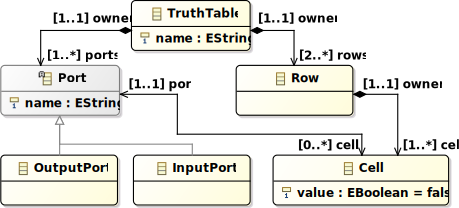
\includegraphics[width=.6\textwidth]{tt-class-diagram-v2}
  \caption{Class diagram for the input Truth Tables metamodel}
  \label{fig:tt-metamodel}
\end{figure}

\begin{table}
  \centering
  \begin{tabular}{llll|l}
    $A$ & $B$ & $C$ & $D$ & $S$ \\
    \hline
    0 & 0 & - & - & 0 \\
    0 & 1 & 0 & 0 & 1 \\
    0 & 1 & 0 & 0 & 1 \\
    0 & 1 & 0 & 1 & 0 \\
    0 & 1 & 1 & - & 0 \\
  \end{tabular}
  \hspace{1em}
  \begin{tabular}{llll|l}
    $A$ & $B$ & $C$ & $D$ & $S$ \\
    \hline
    1 & 0 & 0 & 0 & 0 \\
    1 & 0 & 1 & 0 & 1 \\
    1 & - & - & 1 & 0 \\
    1 & 1 & 0 & 0 & 1 \\
    1 & 1 & 1 & 0 & 0 \\
  \end{tabular}
  \caption{Example truth table: $A$ to $D$ are input ports and $S$ is an output port. ``-'' means ``ignored''.}
  \label{tab:tt-example}
\end{table}

The input metamodel is shown on Figure~\ref{fig:tt-metamodel}. The
\class{Truth\-Table} class is as the root of the model, and contains a
collection of \class{Port}s and \class{Row}s. \class{Port}s come in two types:
\class{Input\-Port}s and \class{Output\-Port}s. \class{Row}s contain sequences
of \class{Cell}s, which assign values to the \class{Input\-Port}s and
\class{Output\-Port}s of the table.

Automated EMF opposite references are used liberally in the metamodel to
simplify the specification of the transformation. \feature{owner} is used to
access the container from several child objects (e.g. the \class{Truth\-Table}
of a \class{Row}), and it is possible to see which \feature{cells} referenced a
specific \class{Port}.

A sample model is shown on Table~\ref{tab:tt-example}. The truth table has four
\class{Input\-Port}s named $A$ to $D$, and one \class{Output\-Port} named $S$.
The first \class{Row} contains only 3 \class{Cell}s, specifying that if $A$ and
$B$ are 0, then $S$ should be 0.

\subsection{Output Metamodel: Binary Decision Trees}
\label{sec:outp-metam-binary}

\begin{figure}[t]
  \centering
  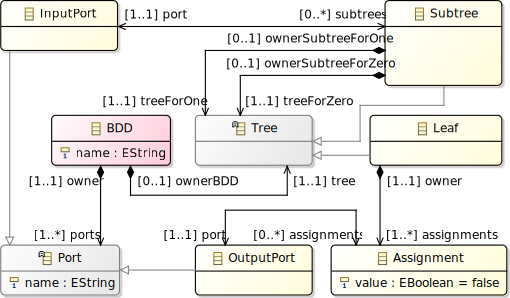
\includegraphics[width=.6\textwidth]{bdd-class-diagram-v2}
  \caption{Class diagram for the output Binary Decision Diagram metamodel, in the original tree-based version.}
  \label{fig:bdd-metamodel}
\end{figure}

\begin{figure}[t]
  \centering
  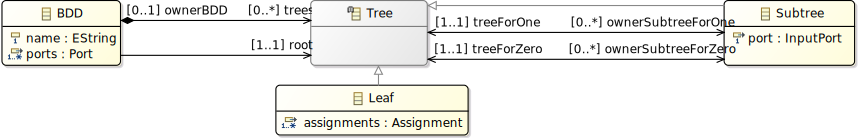
\includegraphics[width=.9\textwidth]{bddg-class-diagram-v2}
  \caption{Changed classes in the graph-based variant of the Binary Decision Diagram metamodel (2019-05-26). Omitted clases remain the same.}
  \label{fig:bddg-metamodel}
\end{figure}

\begin{figure}[t]
  \centering
  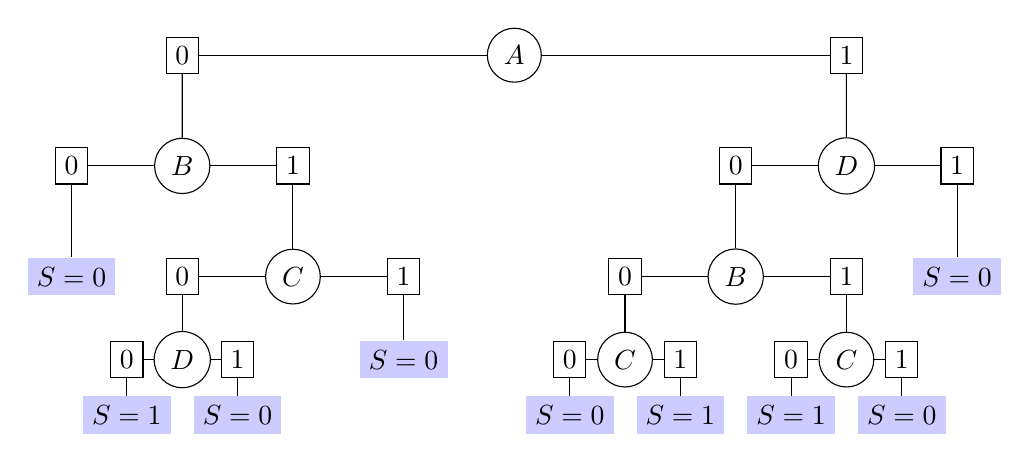
\begin{tikzpicture}[
      level 1/.style={level distance=12em},
      level 2/.style={level distance=4em},
      level 6/.style={level distance=3em},
      level 7/.style={level distance=2em},
      port/.style={circle, draw},
      value/.style={draw},
      assignment/.style={fill=blue!20},
  ]
    \node[port] {$A$}
    child[grow=left] {
      node[value] {0}
      [grow=down]
      child[level distance=4em] {
        node[port] {$B$}
        child[grow=left] {
          node[value] {0}
          child[grow=down] { node[assignment] {$S = 0$} }
        }
        child[grow=right] {
          node[value] {1}
          child[grow=down] {
            node[port] {$C$}
            child[grow=left] {
              node[value] {0}
              child[grow=down] {
                node[port] {$D$}
                child[grow=left] {
                  node[value] {0}
                  child[grow=down] { node[assignment] {$S=1$} }
                }
                child[grow=right] {
                  node[value] {1}
                  child[grow=down] { node[assignment] {$S=0$} }
                }
              }
            }
            child[grow=right] {
              node[value] {1}
              child[grow=down] {node[assignment] {$S=0$}}
            }
          }
        }
      }
    }
    child[grow=right] {
      node[value] {1}
      [grow=down]
      child[level distance=4em] {
        node[port] {$D$}
        child[grow=left] {
          node[value] {0}
          child[grow=down] {
            node[port] {$B$}
            child[grow=left] {
              node[value] {0}
              child[grow=down] {
                node[port] {$C$}
                child[grow=left] {
                  node[value] {0} child[grow=down] { node[assignment] {$S=0$} }
                }
                child[grow=right] {
                  node[value] {1} child[grow=down] { node[assignment] {$S=1$} }
                }
              }
            }
            child[grow=right] {
              node[value] {1}
              child[grow=down] {
                node[port] {$C$}
                child[grow=left] {
                  node[value] {0} child[grow=down] { node[assignment] {$S=1$} }
                }
                child[grow=right] {
                  node[value] {1} child[grow=down] { node[assignment] {$S=0$} }
                }
              }
            }
          }
        }
        child[grow=right] {
          node[value] {1} child[grow=down] { node[assignment] {$S=0$} }
        }
      }
    }
    ;
  \end{tikzpicture}
  \caption{Equivalent BDD for the truth table on Table~\ref{tab:tt-example}.}
  \label{fig:bdd-equivalent}
\end{figure}

The original output metamodel from the ATL Zoo version is shown on
Figure~\ref{fig:bdd-metamodel}. The \class{BDD} class is the root of the model,
and contains the root of the \class{Tree} and a collection of \class{Port}s.
Similarly to the Truth Tables metamodel, there are \class{Input\-Port}s and
\class{Output\-Port}s.

Figure~\ref{fig:bddg-metamodel} shows the changes introduced into a revised
version of the original metamodel, which allow the \class{BDD} to be a rooted
acyclic graph and not just a tree. This would allow the \class{BDD} to reuse
common subtrees, which would produce more compact circuits in some situations.
The case provides both versions as separate metamodels: solution implementers
were free to choose either version.

\class{Tree} is the common superclass for any node in the tree. Inner nodes
check the value of an \class{Input\-Port}: if it is a false value, evaluation
will proceed through the \feature{tree\-For\-Zero} \class{Tree}; otherwise,
evaluation will go through the \feature{tree\-For\-One} \class{Tree}. Leaf nodes
are \class{Leaf} objects, which provide an \class{Assignment} of a boolean value
to each of the available \class{Output\-Port}s.

The equivalent BDD for the truth table on Table~\ref{tab:tt-example} is shown on
Figure~\ref{fig:bdd-equivalent}. \class{Subtree}s are represented by the circle
referencing an \class{Input\-Port} and their subtrees for when the port takes a
0 or 1 value. \class{Assignment}s are represented by the highlighted nodes that
provide values to the \class{Output\-Port}s.

\subsection{Process Outline}
\label{sec:process-outline}

The transformation essentially needs to construct a (preferably minimal) binary
decision diagram that produces the same values for the output ports, given the
same values in the input ports. Given the high interest about this problem in
circuit design, many algorithms have been proposed in the literature.

Solution authors are welcome to implement a more optimal algorithm in their
transformation tool. This section will only outline a simple approach that can
be readily implemented without too much complication.

There are some basic mappings which are immediately obvious:

\begin{itemize}
\item Each \class{TruthTable} object should correspond to a \class{BDD} object,
  with the same name and equivalent \class{Port}s.

\item Each \class{Input\-Port} and \class{Output\-Port} should be mapped to an
  object of the BDD type with the same name.

\item Each \class{Row} should become a \class{Leaf} node: the \class{Cell}s for
  the \class{Output\-Port}s will become \class{Assignment}s.
\end{itemize}

The complexity is in deriving the inner nodes: the \class{Subtree} objects. One
simple approach is to find a TT \class{Input\-Port} which is (ideally) defined
in all the \class{Row}s, and turn it into an inner node (a \class{Subtree})
which points to the equivalent BDD \class{Input\-Port} and has two
\class{Tree}s:
\begin{itemize}
\item The zero subtree, produced from the \class{Row}(s) where the port was 0.
  This will be a \class{Subtree} if there are at least two rows in that
  situation: the transformation should proceed recursively in this case with
  those rows, excluding the input ports that have already been considered. If
  there is only one such row, this would simply point to the \class{Leaf}
  created above.

\item The one subtree, produced in a parallel way to the zero subtree.
\end{itemize}

This simple approach does not necessarily ensure a minimal subtree, as in some
points there may be multiple ports to choose from. It may require improvements
for cases where there are no input ports which are defined in all available
rows.

\section{Main Task}
\label{sec:task-suggestions}

The main task was implementing the transformation, ensuring that the BDDs were
equivalent to the original truth table. To simplify the work involved, the case
included an Eclipse Modelling Framework implementation, and a set of sample XMI
input models conforming to the metamodels.

The \file{models} folder includes two additional tools:
\begin{itemize}
\item A generator that produced truth tables of an arbitrary number of input and
  output ports, given a seed.

\item A validator that checked if a BDD model was equivalent to a source truth
  table model, by evaluating all possible input combinations through the BDD and
  comparing the values of the \class{Output\-Port}s.
\end{itemize}

Solutions could focus on any specific quality attribute of the transformation
beyond optimality and performance. For instance, it may be useful to be able to
prove that the transformation does indeed produce a BDD which is equivalent to
the TT (even if suboptimal). One of the solutions did focus on verifiability.

\section{Benchmark Framework}
\label{sec:benchmark-framework}

If focusing on performance, the solution authors had to integrate their solution
with the provided benchmark framework. It is based on that of the TTC 2017 Smart
Grid case~\cite{hinkel_ttc_2017}, and supports the automated build and execution
of solutions. The framework consists of a Python 3.3 script which directs the
process, and a set of R scripts which perform basic data analysis and reporting.

The benchmark consisted of three phases: \textbf{Initialisation} (setting up the
basic infrastructure), \textbf{Load} (for loading the models), and \textbf{Run}
(for executing the transformation and saving the results).

Solutions had to be forks of the main Github
project\footnote{\url{https://github.com/TransformationToolContest/ttc2019-tt2bdd}},
for their later integration into the main Github repository. The solutions could
be implemented in any language: they only had to print to the standard output
lines in a specific format, mentioning the memory usage and wall clock time
spent in transforming each model.

The solutions had to include a \file{solution.ini} file with instructions on how
to automatically build, test, and run them. Solutions were run multiple times,
as indicated in the main configuration of the benchmark. To ensure
reproducibility, the solutions were integrated into a Docker image, which is
automatically built by Docker Hub on each
push\footnote{\url{https://hub.docker.com/r/bluezio/ttc2019-tt2bdd-git}}.

\section{Evaluation}
\label{sec:evaluation}

Given the call for a broader set of research interests in this transformation,
the evaluation operated on two dimensions:

\begin{itemize}
\item Was it a high-quality model transformation? The transformation should be
  complete, correct, easy to understand, efficient, and produce optimal results.

  The validator was used to check the produced BDDs against the source truth
  tables, and the authors had to provide a convincing argument about the
  correctness of the solution.

  The understandability of the solution was evaluated through an audience
  survey, and the Docker image was used by the contest organizers to provide
  independent measurements of memory and time usage in identical conditions.
  Particularly, Google Cloud Compute \file{c2-standard-4} images were used.

  Tree sizes for the BDDs were considered for the optimality of the
  transformations: the smaller, the better.

\item Did it highlight a promising research direction? Although the
  transformation may not be entirely complete or may be harder to understand, it
  may serve as an example of an active research area within model
  transformations that the community may wish to showcase.

  This may include aspects such as incrementality, bidirectionality,
  traceability, verifiability, or the ability to visualize interactively the
  transformation, among other areas of interest in the field.

  As mentioned before, there was one solution which focused on the verifiability
  of the solution. This solution received an award for the promising results
  towards integrating verifiability in a model transformation language.
\end{itemize}

\bibliographystyle{plain}
\bibliography{bibliography}

\end{document}
